\documentclass[../main.tex]{subfiles}
\begin{document}

\graphicspath{{../imagenes/}{imagenes/}}

\chapter{Pipeline de inferencia de radiografías y generación de informes}
\label{cap:Capitulo5}

\section{Diseño del flujo de trabajo}
\label{sec:Diseño del flujo de trabajo}
Al evaluar la viabilidad de distintos modelos de Inteligencia Artificial a lo largo de este trabajo, se identificó la oportunidad de integrar múltiples arquitecturas en un único flujo de trabajo orientado al análisis de radiografías y a la generación de informes radiológicos. En particular, se diseñó un \textit{pipeline} (\autoref{fig:flujo_sistema}) estructurado en tres bloques principales:
\begin{enumerate}
    \item Un modelo de clasificación binaria que analiza la imagen y determina si corresponde a un estado normal o patológico.
    \item Un modelo clasificador multietiqueta que, en caso de detectarse una anomalía, evalúa la presencia de una o varias de las 14 patologías posibles.
    \item Un Modelo de Lenguaje de Gran Escala (LLM) que redacta un informe radiológico completo a partir de los hallazgos de los modelos previos e información contextual del paciente (metadatos, historial clínico, síntomas, entre otros).
\end{enumerate}
\begin{figure}[htbp]
    \centering
    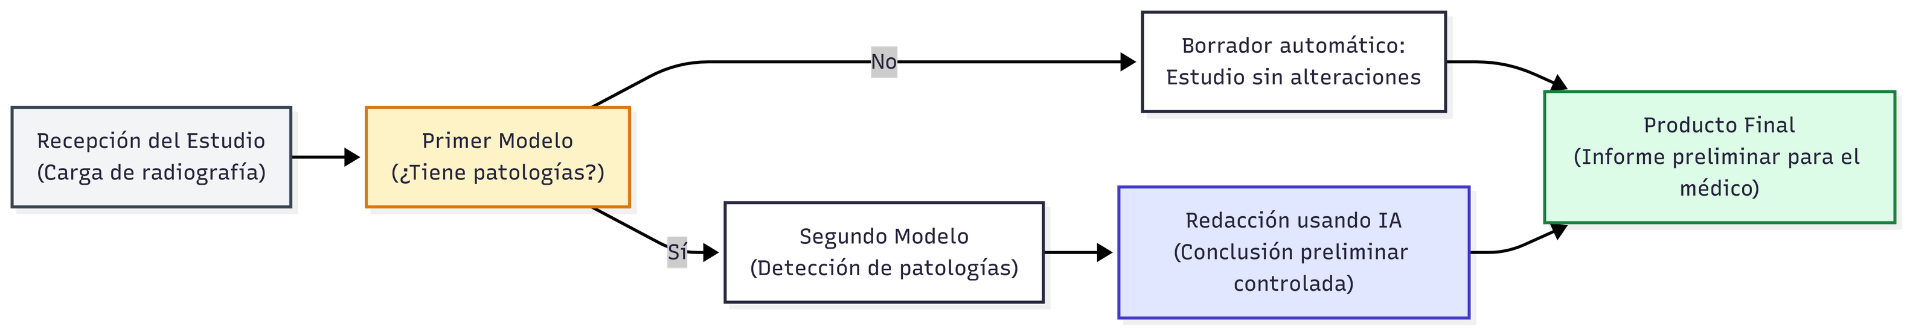
\includegraphics[width=1.1\textwidth]{Tesis/Presentacion Lavalle 11.png}
    \caption{Diagrama de flujo conceptual del sistema CAD.}
    \label{fig:flujo_sistema}
\end{figure}
Dado que los modelos preentrenados evaluados en las etapas iniciales mostraron un rendimiento limitado sobre el conjunto de datos local, se decidió reentrenar y ajustar las redes utilizando tanto la base de datos propia como repositorios públicos de radiografías etiquetadas. Para reforzar el conjunto de entrenamiento, se incorporó el dataset de acceso público \textit{NIH Chest X-rays} \citep{nih_chest_xrays_kaggle}, el cual consta de $112\,120$ radiografías de tórax pertenecientes a $30\,805$ pacientes, etiquetadas en 15 categorías.

\section{Estructura de Entrenamiento}

\subsection{Arquitectura de Red y Estrategia de Pesos Base}
El entrenamiento parte de los pesos estandarizados provistos por la biblioteca TorchXRayVision (XRV) bajo el identificador \texttt{resnet50-res512-all} \citep{Cohen2020xrv}. Se trata de una red neuronal convolucional basada en la arquitectura ResNet-50, optimizada para procesar imágenes médicas a una resolución de $512 \times 512$ píxeles y preentrenada sobre múltiples conjuntos de datos internacionales de radiografías de tórax. Esta constituye la variante de mayor resolución disponible en XRV.

Dado que el modelo base \texttt{resnet50-res512-all} ya incluye al dataset NIH en su preentrenamiento global, la evaluación posterior sobre NIH no constituye una validación externa independiente, sino una verificación interna sobre un benchmark público conocido. El ajuste fino (\textit{fine-tuning}) supervisado sobre NIH se realizó con el propósito de adaptar los pesos a las convenciones de etiquetado y calibrar los umbrales de decisión mediante el índice de Youden, reservando a la cohorte local como la verdadera prueba de generalización externa (si bien sujeta a las limitaciones propias del etiquetado automático).

\subsection{Preprocesamiento, Carga y Estandarización de Datos}
\label{sec:Preprocesamiento, Carga y Estandarización de Datos}
El pipeline de ingesta y preprocesamiento de imágenes fue diseñado para resolver la alta heterogeneidad inherente a la combinación de bases de datos públicas internacionales (como NIH, en formatos estándar) y repositorios clínicos locales (con imágenes DICOM propietarias). Para ello, se implementó un flujo unificado compatible con la red neuronal:

\begin{enumerate}
    \item \textbf{Ingesta diferenciada por formato:} El sistema procesa dinámicamente las imágenes según su extensión de origen:
    \begin{itemize}
        \item \textbf{Imágenes estándar de 8 bits (\texttt{.png}, \texttt{.jpg}):} Predominantes en el dataset NIH, se cargan mediante la biblioteca PIL convirtiéndolas a escala de grises (\texttt{Image.open().convert("L")}) y se transforman en arreglos numéricos de punto flotante.
        \item \textbf{Imágenes médicas DICOM (\texttt{.dcm}):} Procedentes del entorno local, se procesan extrayendo sus píxeles crudos. Si presentan tres canales (RGB), se convierten a escala de grises (\texttt{cv2.cvtColor}). Si se detecta una interpretación fotométrica invertida (\texttt{MONOCHROME1}), los valores se invierten linealmente para preservar la semántica visual estándar (aire pulmonar oscuro y estructuras densas claras).
    \end{itemize}
    
    \item \textbf{Normalización de profundidad de bits y ventana DICOM:} Para corregir las disparidades en la resolución radiométrica del flujo DICOM (8 bits frente a 12 o 16 bits de alta profundidad), se implementó un ajuste dinámico:
    \begin{itemize}
        \item Para archivos de profundidad $\le 8$ bits, se aplica una normalización lineal min-max al rango $[0, 255]$.
        \item Para archivos de alta profundidad, se extraen los metadatos de centro (\texttt{WindowCenter}) y ancho de ventana (\texttt{WindowWidth}), realizando un recorte (\textit{clipping}) del rango de interés clínico seguido de su reescalado a 8 bits.
    \end{itemize}
    
    \item \textbf{Mejora local de contraste (CLAHE):} Una vez unificadas las imágenes en un formato matricial base, se aplicó el algoritmo de Ecualización de Histograma Adaptativo Limitado por Contraste (\textit{CLAHE}) \citep{Zuiderveld1994}. Configurado con un límite de contraste ($\text{clipLimit} = 2.0$) y una rejilla de $8 \times 8$ bloques, este paso realza bordes sutiles y detalles anatómicos de baja frecuencia tanto en las radiografías DICOM locales como en las del NIH.
    
    \item \textbf{Transformaciones espaciales y resolución fija:} Para cumplir con los requerimientos de la arquitectura ResNet-50 a una resolución de $512 \times 512$ píxeles, las imágenes se redimensionan manteniendo su proporción mediante un escalado del lado menor a 512 píxeles (\texttt{transforms.Resize}), seguido de un recorte central (\texttt{transforms.CenterCrop}). Exclusivamente para el conjunto de entrenamiento, se aplicaron técnicas de aumento de datos (\textit{data augmentation}) moderadas:
    \begin{itemize}
        \item Transformaciones afines aleatorias (\texttt{RandomAffine}) con rotaciones de hasta $\pm 7^\circ$, traslaciones del $2\%$ y reescalados entre $0.95$ y $1.05$.
        \item Variaciones de contraste ($15\%$) y brillo ($10\%$) mediante \texttt{ColorJitter}.
    \end{itemize}
    
    \item \textbf{Estandarización de intensidad para TorchXRayVision:} Tras convertir las imágenes en tensores normalizados en el rango $[0, 1]$, se aplicó la transformación de escala específica requerida por los pesos preentrenados de \textit{TorchXRayVision}:
    $$\text{Imagen}_{\text{XRV}} = \text{Tensor} \times 2048.0 - 1024.0$$
    Este mapeo traslada la distribución al intervalo $[-1024, 1024]$, garantizando la compatibilidad numérica exacta con las características estadísticas aprendidas por la red base.
\end{enumerate}

\subsection{Aprendizaje Autosupervisado (SSL) para Adaptación de Dominio}
\label{Seccion SSL}

Con el objetivo de mitigar el desplazamiento de dominio (\textit{domain shift}) entre los repositorios internacionales y la distribución local, se implementó una fase inicial de Aprendizaje Autosupervisado (SSL) previa al ajuste fino supervisado. Este proceso permitió que el extractor de características adaptara sus representaciones latentes a las particularidades de las imágenes locales sin requerir etiquetas diagnósticas.

Tal como se detalló en las secciones correspondientes, solo una fracción del dataset local contaba con etiquetas aptas para el entrenamiento supervisado. En consecuencia, se utilizaron 14132 radiografías de tórax (proyecciones PA o AP) no etiquetadas para conformar el conjunto de entrenamiento SSL. A partir del registro de rutas (\texttt{ssl\_dataset\_paths.csv}), los datos se dividieron aleatoriamente en un conjunto de entrenamiento (85\%) y uno de validación (15\%), con semilla fija (\texttt{random\_state} $= 42$). Previamente, se excluyeron de forma estricta todos los identificadores de pacientes presentes en el conjunto de evaluación mediante el cruce con el repositorio de etiquetas (\texttt{labels\_extraidas\_informes.json}), garantizando que ninguna radiografía destinada al preentrenamiento autosupervisado perteneciera a las cohortes de prueba o validación supervisada. Dicha separación libre de solapamientos se validó programáticamente mediante la verificación de intersección nula entre los conjuntos de identificadores únicos de pacientes de cada partición (asegurando la condición de conjuntos disjuntos, \texttt{isdisjoint}), evitando así cualquier filtración de información (\textit{data leakage}).

Para el desarrollo del experimento se establecieron los siguientes aspectos metodológicos:

\begin{enumerate}
    \item \textbf{Arquitectura del modelo:} Se diseñó un \textit{autoencoder} basado en la ResNet-50 de \textit{TorchXRayVision}. El codificador (\textit{encoder}) reutiliza las capas convolucionales profundas del modelo base (\texttt{layer1} a \texttt{layer4}), generando un mapa de características latentes de 2048 canales. Por su parte, el decodificador simétrico consta de cinco capas de convolución transpuesta (\texttt{nn.ConvTranspose2d}) intercaladas con activaciones ReLU, las cuales reconstruyen gradualmente la imagen de entrada a una resolución de $512 \times 512$ píxeles y un solo canal de salida.

    \item \textbf{Configuración del entrenamiento:} La optimización se enfocó en la reconstrucción fiel de las imágenes mediante las siguientes estrategias:
    \begin{itemize}
        \item \textbf{Función de pérdida:} Se empleó el Error Cuadrático Medio (MSE) para penalizar las discrepancias a nivel de píxel:
        $$\mathcal{L}_{\text{SSL}} = \text{MSE}(\hat{X}, X)$$
        \item \textbf{Optimizador y tasa de aprendizaje:} Se utilizó el algoritmo Adam con una tasa de aprendizaje constante de $1 \times 10^{-4}$.
        \item \textbf{Eficiencia computacional:} Ante las restricciones de VRAM, se configuró un tamaño de lote físico de 8 muestras con acumulación de gradientes (4 pasos), simulando un lote efectivo de 32 muestras. Se empleó precisión mixta (\texttt{torch.amp.GradScaler} y \texttt{torch.autocast}) para optimizar el uso de memoria.
        \item \textbf{Criterios de parada:} El entrenamiento se ejecutó durante un máximo de 20 épocas, empleando un mecanismo de \textit{Early Stopping} con una paciencia de 4 épocas monitoreada sobre la pérdida de validación. Los mejores pesos se almacenaron en \texttt{backbone\_ssl\_local.pth} para inicializar las etapas supervisadas.
    \end{itemize}
\end{enumerate}

El preentrenamiento autosupervisado completó de forma íntegra las 20 épocas configuradas, convergiendo hacia un error cuadrático medio (MSE) de validación final de 12334,46 en la época 20, momento en el cual se almacenaron los pesos definitivos en el archivo \texttt{backbone\_ssl\_local.pth}.

\subsection{Fine-Tuning Supervisado (SFT) y Optimización de Clasificación}

Completada la etapa de adaptación de dominio con SSL, el modelo se sometió a un proceso de \textit{Fine-Tuning} Supervisado (SFT). En esta fase se adaptaron los pesos del \textit{backbone} para resolver tareas clínicas específicas mediante la incorporación de capas de clasificación especializadas.

Para garantizar la reproducibilidad y el rigor metodológico en las fases de ajuste fino supervisado (SFT), la gestión de los conjuntos de datos se estructuró mediante archivos de partición explícitos y versionados. Dado que el entrenamiento supervisado de los modelos discriminativos se ejecutó exclusivamente sobre el repositorio público NIH Chest X-ray14, las muestras de entrenamiento y validación se administraron mediante archivos dedicados (como \texttt{train\_nih.csv} y \texttt{val\_nih.csv} para el modelo binario, y \texttt{train\_etapa2.csv} y \texttt{val\_etapa2.csv} para el modelo multietiqueta), la división entre entrenamiento y validación se ejecutó estrictamente a nivel de paciente (\texttt{Clean\_Patient\_ID}) utilizando una semilla fija (\texttt{random\_state} $= 42$). Esta estrategia impidió que múltiples proyecciones o estudios de un mismo individuo quedaran repartidos simultáneamente en ambas particiones, previniendo sesgos por sobreajuste y garantizando la independencia estadística de las evaluaciones. Por su parte, la cohorte clínica local se mantuvo completamente aislada del entrenamiento supervisado y se reservó de manera estricta para el preentrenamiento autosupervisado en su componente no etiquetado (mediante \texttt{ssl\_dataset\_paths.csv}) y para la evaluación ciega de generalización externa (mediante \texttt{test\_local\_split.csv} y \texttt{test\_local.csv}), garantizando así una auditoría rigurosa frente al desplazamiento de dominio (\textit{domain shift}).



\subsubsection{Clasificación Binaria (Normal vs. Patológico)}
Para la clasificación binaria, se reemplazó la capa totalmente conectada final por una única salida lineal ($n_{out}=1$), inicializando la red con los pesos aprendidos en el autoencoder SSL (\texttt{backbone\_ssl\_local.pth}). El entrenamiento y la validación supervisada de este módulo se ejecutaron cargando los registros estructurados en \texttt{train\_nih.csv} y \texttt{val\_nih.csv} sobre el dataset NIH Chest X-ray14. Para compensar el desbalance de clases, se utilizó la función de pérdida de entropía cruzada binaria con logits (\texttt{BCEWithLogitsLoss}), ponderando la clase positiva mediante el parámetro \texttt{pos\_weight} calculado sobre las etiquetas de entrenamiento:
\begin{equation}
\text{pos\_weight} = \frac{N_{\text{negativos}}}{N_{\text{positivos}}}
\end{equation}
El entrenamiento se configuró a 20 épocas utilizando el optimizador Adam con una tasa de aprendizaje de $1\times10^{-4}$, un tamaño de lote efectivo de 32 (lote físico de 8 muestras con acumulación de gradientes en 4 pasos) y precisión mixta de 16 bits mediante \texttt{GradScaler}. La selección del mejor punto de control (\textit{checkpoint}) se basó en el monitoreo del área bajo la curva ROC (AUC-ROC) sobre el conjunto de validación definido en \texttt{val\_nih.csv}, aplicando una parada temprana (\textit{early stopping}) tras 4 épocas sin mejora en la pérdida. Finalmente, la evaluación ciega de generalización externa se procesó sobre la cohorte local definida en \texttt{test\_local\_split.csv}.

\subsubsection{Optimización de Umbrales (Threshold Tuning)}
Dado que el umbral de decisión predeterminado de $0.5$ suele ser subóptimo en escenarios con desbalance de clases, se realizó una calibración posterior sobre el conjunto de validación de NIH. 

A partir de las probabilidades predichas $\hat{y} = \sigma(z)$ y las etiquetas reales, se analizó la curva ROC y se seleccionó el umbral óptimo $t^*$ mediante la maximización del índice $J$ de Youden:
\begin{equation}
    J(t) = \text{TPR}(t) - \text{FPR}(t) = \text{Sensibilidad}(t) + \text{Especificidad}(t) - 1
\end{equation}
\begin{equation}
    t^* = \arg\max_{t} J(t)
\end{equation}

El umbral derivado empíricamente ($t^* \approx 0.3999$) se fijó de manera definitiva para la etapa de inferencia sobre el conjunto de datos local.

\subsubsection{Clasificación Multietiqueta (14 Clases)}
Para extender la capacidad diagnóstica a patologías específicas, se desarrolló un segundo modelo SFT orientado a clasificación multietiqueta sobre las 14 categorías del estándar NIH. Utilizando los archivos de partición \texttt{train\_etapa2.csv} y \texttt{val\_etapa2.csv} para el ajuste y validación sobre el repositorio público, y el archivo \texttt{test\_local.csv} para la evaluación de generalización externa con la totalidad de la cohorte local.

Sobre el mismo \textit{backbone} inicializado con SSL, se ajustó la capa de salida a un vector de 14 dimensiones. En esta etapa se introdujeron las siguientes modificaciones para regularizar el entrenamiento:
\begin{itemize}
    \item \textbf{Optimizador y regularización:} Se sustituyó Adam por \textbf{AdamW} con un decaimiento de peso (\textit{weight decay}) de $10^{-2}$.
    \item \textbf{Planificación de la tasa de aprendizaje:} Se implementó un programador de tipo \textit{Cosine Annealing} (\texttt{CosineAnnealingLR}) para decrecer suavemente la tasa de aprendizaje.
    \item \textbf{Restricción de pesos de clase (\textit{Clamping}):} Los factores de penalización por clase (\textit{pos\_weights}) se acotaron a un valor máximo de $10.0$ ($\max = 10.0$) para evitar la dominancia de clases extremadamente minoritarias en el gradiente.
    \item \textbf{Métrica de evaluación e inferencia:} Se evaluó el rendimiento mediante el AUC Macro (\textit{Macro-averaged ROC-AUC}) sobre las 14 clases, aplicando parada temprana con una paciencia de 5 épocas.
\end{itemize}

\section{Resultados de Validación y Evaluación Externa (Test)}

En esta sección se presentan los resultados obtenidos en la verificación interna sobre el benchmark público conocido NIH Chest X-ray14 —cuyos datos forman parte del preentrenamiento del modelo base de TorchXRayVision— y en la evaluación de generalización externa sobre la cohorte local independiente ($N=563$ para clasificación binaria y $N=592$ para multietiqueta).

\subsection{Modelo de Clasificación Binaria (Normal vs. Patológico)}

El modelo binario operó bajo el umbral óptimo $t^* = 0.3999$, determinado con el Índice de Youden en la cohorte NIH. La \autoref{tab:resultados_binarios} resume las métricas alcanzadas.


\begin{table}[htbp]
    \centering
    \begin{tabular}{lcc}
        \toprule
        \textbf{Métrica} & \textbf{Validación NIH} & \textbf{Test Local} \\
        \midrule
        Muestras totales ($N$) & 22\,294 & 563 \\
        Pérdida (\textit{BCE Loss}) & 0.6301 & -- \\
        \textbf{AUC-ROC} & \textbf{0.7679} & \textbf{0.7640} \\
        Sensibilidad / \textit{Recall} (Patológico) & 0.7358 & 0.6695 \\
        Especificidad / \textit{Recall} (Normal) & 0.6851 & 0.7393 \\
        Valor Predictivo Positivo (VPP / \textit{Precision}) & 0.6676 & 0.4100 \\
        Valor Predictivo Negativo (VPN) & 0.7509 & 0.8940 \\
        \textit{F1-Score} (Clase Patológica) & 0.6999 & 0.5000 \\
        Exactitud Global (\textit{Accuracy}) & 0.7085 & 0.7247 \\
        Umbral de decisión ($t^*$) & 0.3999 & 0.3999 (fijado) \\
        \bottomrule
    \end{tabular}
    \caption{Desempeño del modelo binario en validación interna (NIH) y test externo (Dataset Local) con $t^* = 0.3999$.}
    \label{tab:resultados_binarios}
\end{table}

\subsubsection{Matriz de Confusión y Análisis de Generalización Binaria}
Las matrices de confusión resultantes se muestran en la \autoref{fig:matriz_confusion}.
\begin{figure}[htbp]
\centering
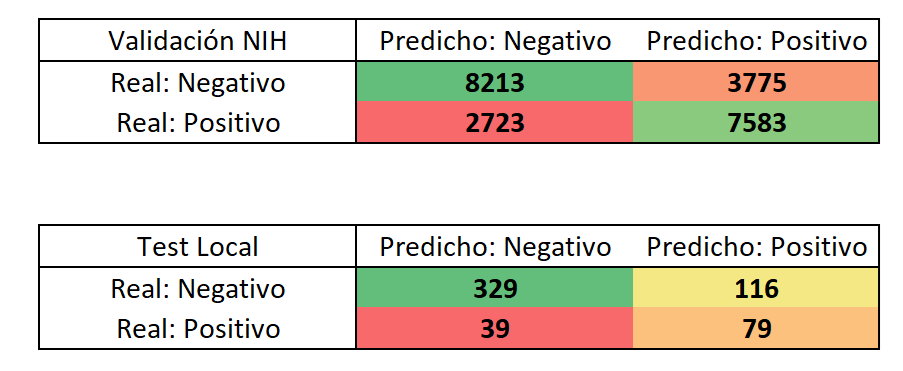
\includegraphics[width=0.8\textwidth]{Tesis/Matriz de confusion.png}
\caption{Comparativa de matrices de confusión ($2 \times 2$) representadas como mapas de calor para los conjuntos de validación NIH y prueba local.}
\label{fig:matriz_confusion}
\end{figure}

\paragraph{Discusión de la clasificación binaria:} 
El modelo mostró una capacidad discriminativa altamente consistente, alcanzando un área bajo la curva ROC en la cohorte local ($AUC-ROC = 0{,}7640$) comparable a la obtenida en la verificación interna sobre NIH ($AUC-ROC = 0{,}7679$) \autoref{fig:domain_shift_binario}. Dado que NIH está incluido en el preentrenamiento de TorchXRayVision, su evaluación funciona como una validación interna sobre un benchmark conocido, mientras que la verdadera prueba de transferencia y generalización externa recae en el desempeño sobre el dataset local. No obstante, la caída observada en el Valor Predictivo Positivo ($0{,}4100$) responde a la alta proporción de casos normales en la cohorte local ($79{,}0\%$), por lo que este desarrollo se mantiene como un prototipo de investigación no validado para uso clínico autónomo.
\begin{figure}[htbp]
\centering
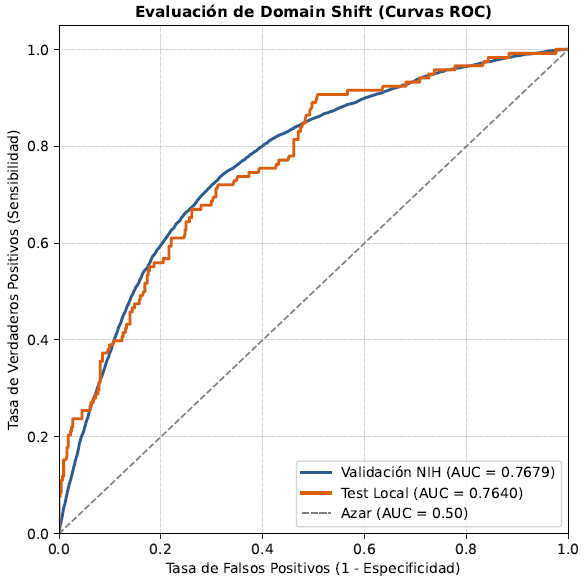
\includegraphics[width=0.6\textwidth]{Tesis/domain_shift_binario.png}
\caption{Curvas ROC superpuestas del modelo binario: validación NIH ($AUC = 0.7679$) frente a test local ($AUC = 0.7640$).}
\label{fig:domain_shift_binario}
\end{figure}
Esto confirma que las representaciones visuales extraídas tras la fase SSL son robustas frente al desplazamiento de dominio provocado por las diferencias técnicas de adquisición entre centros \citep{Drukker_et_al._2023}.

Por otra parte, la caída observada en el Valor Predictivo Positivo en el test local ($0.4100$) responde a la alta proporción de casos normales en dicha cohorte ($79{,}0\%$, $445/563$). Bajo este escenario de prevalencia negativa, un número reducido de falsos positivos impacta sustancialmente sobre el VPP, aunque la sensibilidad diagnóstica se mantiene en un nivel aceptable ($66.95\%$).

\subsection{Modelo de Clasificación Multietiqueta (14 Patologías)}

Para la clasificación multietiqueta, se determinaron umbrales óptimos independientes por patología sobre la validación de NIH ($N = 5176$). Estos se fijaron y aplicaron directamente durante la inferencia en el conjunto local ($N = 592$). La \autoref{tab:multilabel_results} detalla los resultados por categoría mientras que la \autoref{fig:barras_laterales} compara las métricas de forma visual.

\begin{table}[htbp]
    \centering
    \scriptsize
    \begin{tabular}{l | cc c | cc c c}
        \toprule
        & \multicolumn{3}{c|}{\textbf{Validación NIH ($N=5176$)}} & \multicolumn{4}{c}{\textbf{Test Local ($N=592$)}} \\
        \textbf{Patología} & \textbf{Pos.} & \textbf{AUC} & \textbf{Umbral ($t^*$)} & \textbf{Pos.} & \textbf{AUC} & \textbf{Sens.} & \textbf{Espec.} \\
        \midrule
        Atelectasis          & 1153 & 0.7664 & 0.4846 & 23  & 0.6705 & 0.4348 & 0.8576 \\
        Cardiomegaly         & 263  & 0.8955 & 0.4355 & 310 & \textbf{0.9340} & 0.5452 & 0.9574 \\
        Consolidation        & 471  & 0.6956 & 0.4648 & 71  & 0.7196 & 0.0845 & 0.9846 \\
        Edema$^{\dagger}$    & 233  & 0.8515 & 0.2496 & 5   & n/d    & n/d    & n/d    \\
        Effusion             & 1337 & 0.8288 & 0.4795 & 52  & 0.7191 & 0.4808 & 0.8926 \\
        Emphysema            & 275  & 0.9139 & 0.3159 & 17  & 0.8720 & 0.7647 & 0.7374 \\
        Fibrosis             & 167  & 0.8189 & 0.3003 & 37  & 0.6850 & 0.8649 & 0.3009 \\
        Hernia               & 24   & 0.9276 & 0.0464 & 13  & 0.7722 & 0.8462 & 0.5181 \\
        Infiltration         & 2017 & 0.6941 & 0.5205 & 47  & 0.6151 & 0.4043 & 0.7596 \\
        Mass$^{\dagger}$     & 565  & 0.8092 & 0.5195 & 1   & n/d    & n/d    & n/d    \\
        Nodule               & 641  & 0.7423 & 0.4785 & 20  & 0.6944 & 0.9500 & 0.1224 \\
        Pleural Thickening   & 334  & 0.7067 & 0.4084 & 50  & 0.6335 & 0.8000 & 0.2749 \\
        Pneumonia            & 145  & 0.6545 & 0.1869 & 67  & 0.5603 & 0.3881 & 0.7010 \\
        Pneumothorax$^{\dagger}$ & 476 & 0.8446 & 0.4980 & 4   & n/d    & n/d    & n/d    \\
        \bottomrule
    \end{tabular}
    \\[1ex]
    \caption{Resultados del modelo multietiqueta en Validación (NIH) y Test Externo (Local).}
    \label{tab:multilabel_results}
    \raggedright \textit{Nota:} $^{\dagger}$Patologías con un número crítico de muestras positivas ($N \le 5$) en la cohorte de prueba local. Sus métricas se omiten y reportan como no determinables (n/d) por carecer de representatividad y estabilidad estadística.
\end{table}

\begin{figure}[htbp]
\centering
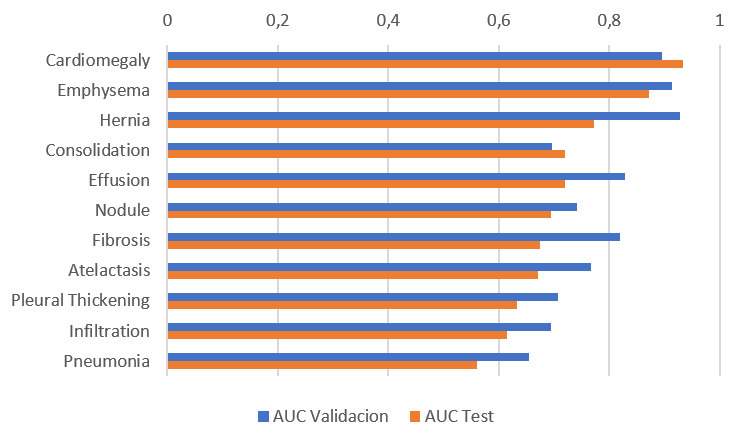
\includegraphics[width=0.8\textwidth]{Tesis/barras laterales.png}
\caption{Comparación del área bajo la curva (AUC) por patología entre el conjunto de validación NIH y la cohorte de prueba externa local, ordenadas de mayor a menor rendimiento en el entorno local.}
\label{fig:barras_laterales}
\end{figure}

\subsubsection{Análisis Clínico-Radiológico del Modelo Multietiqueta}

\begin{enumerate}
    \item \textbf{Patologías con excelente generalización:} Los hallazgos con patrones anatómicos delimitados, como \textit{Cardiomegaly}, mantuvieron un desempeño sobresaliente al evaluarse en la cohorte local, con un $\text{AUC-ROC} = 0.9340$ (frente al $0.8955$ de NIH). Del mismo modo, alteraciones estructurales focalizadas como \textit{Emphysema} ($\text{AUC} = 0.8720$) y \textit{Hernia} ($\text{AUC} = 0.7722$) conservaron una alta capacidad discriminativa.
    
    \item \textbf{Patologías difusas y variabilidad interobservador:} Hallazgos con patrones radiológicos difusos o de interpretación subjetiva —como \textit{Infiltration} ($\text{AUC} = 0.6151$) y \textit{Pneumonia} ($\text{AUC} = 0.5603$)— sufrieron una degradación en el AUC durante la prueba externa. Esto concuerda con lo reportado en la literatura médica \citep{irvin2019chexpertlargechestradiograph}, donde se señala que la discrepancia entre las etiquetas extraídas mediante NLP (en NIH) y las lecturas locales de confirmación incrementa el solapamiento entre hallazgos como consolidaciones e infiltrados.
    
    \item \textbf{Limitaciones por baja prevalencia local:} Las categorías \textit{Edema} ($N=5$), \textit{Pneumothorax} ($N=4$) y \textit{Mass} ($N=1$) contaron con una presencia escasa en la cohorte local de prueba. En consecuencia, sus estimaciones puntuales de sensibilidad y AUC presentan intervalos de confianza amplios y deben interpretarse con reserva.
\end{enumerate}

\section{Pipeline Integrado de Inferencia y Generación de Informes Radiológicos}
\label{sec:pipeline_inferencia}

Para la generación automatizada de borradores de informes radiológicos, se implementó un \textit{pipeline} en cascada modularizado en tres etapas: preprocesamiento, clasificación jerárquica con dos redes ResNet-50 en serie y síntesis de lenguaje clínico mediante un LLM ejecutado localmente.

\subsection{Preprocesamiento Unificado de Imágenes}
Para asegurar la coherencia con el entrenamiento, la ingesta acepta archivos DICOM (\texttt{.dcm}) e imágenes convencionales (\texttt{.png}, \texttt{.jpg}), ejecutando la siguiente secuencia:

\begin{enumerate}
    \item \textbf{Normalización DICOM y tratamiento fotométrico:} En imágenes con \texttt{MONOCHROME1}, se invierten las intensidades ($I' = I_{\max} - I$). Si la profundidad excede los 8 bits ($\text{BitsStored} > 8$), se aplica un reescalado de ventana basado en el centro ($WC$) y ancho ($WW$):
    \begin{equation}
        I_{\text{win}}(x,y) = \text{clip}\left( \frac{I(x,y) - (WC - WW/2)}{WW}, 0, 1 \right) \times 255
    \end{equation}
    De no disponer de dichos metadatos o ante profundidades de 8 bits, se realiza una normalización Min-Max.
    
    \item \textbf{Ecualización adaptativa de histograma (CLAHE):} Se aplica CLAHE con un límite de contraste de $2.0$ y rejilla de $8 \times 8$ sobre la imagen resultante en 8 bits.
    
    \item \textbf{Ajuste espacial y de rango:} La imagen se redimensiona y recorta al centro a $512 \times 512$ píxeles, reescalando posteriormente el tensor al intervalo $[-1024, 1024]$ requerido por TorchXRayVision:
    \begin{equation}
        T_{\text{in}} = T_{\text{tensor}} \cdot 2048.0 - 1024.0
    \end{equation}
\end{enumerate}

\subsection{Cascada de Clasificación Visual (Etapas 1 y 2)}
El módulo de visión por computadora opera mediante un filtrado condicional en dos etapas para optimizar tiempo de cómputo y reducir falsos positivos:

\begin{description}
    \item[Etapa 1 (Filtro Binario de Anormalidad):] El tensor $T_{\text{in}}$ es evaluado por el modelo binario. La probabilidad predicha $p_{\text{bin}} = \sigma(f_{\text{bin}}(T_{\text{in}}))$ se compara con el umbral calibrado ($\tau_{\text{bin}} = 0.3999$):
    \begin{equation}
        \text{Estado}_{\text{bin}} = \begin{cases} 
            \text{Patológico}, & \text{si } p_{\text{bin}} \ge 0.3999 \\ 
            \text{Sin Alerta}, & \text{si } p_{\text{bin}} < 0.3999 
        \end{cases}
    \end{equation}
    Si la probabilidad no supera el umbral, el sistema interrumpe la evaluación multietiqueta y emite directamente un reporte de estudio sin alteraciones.

    \item[Etapa 2 (Clasificación Multietiqueta y Jerarquización):] Si se activa la alerta binaria, el tensor pasa a la red multietiqueta para evaluar las $K=14$ patologías. Las probabilidades $p_c = \sigma(f_{\text{multi}, c}(T_{\text{in}}))$ se comparan contra los umbrales específicos $\tau_c$. Las clases detectadas ($p_c \ge \tau_c$) se estratifican en dos niveles de confianza clínica:
    \begin{itemize}
        \item \textbf{Hallazgos de mayor respaldo (prioritarios):} Clases con mayor sensibilidad operativa en el entrenamiento (p. ej., \textit{Cardiomegalia, Consolidación, Derrame Pleural, Edema, Enfisema, Neumotórax}).
        \item \textbf{Señales exploratorias:} Patologías secundarias o con mayor variabilidad diagnóstica (\textit{Atelectasia, Infiltrado, Masa, Nódulo, Neumonía}, entre otras).
    \end{itemize}
\end{description}

\subsection{Generación Controlada del Informe Radiológico mediante LLM}
La tercera etapa integra los hallazgos de visión y los metadatos del paciente para redactar la conclusión del informe. Para ello se utiliza el modelo de lenguaje \texttt{Qwen2.5:7b}, desplegado localmente mediante Ollama.

A fin de prevenir alucinaciones clínicas y garantizar la reproducibilidad del sistema, se diseñó la siguiente estrategia de redacción restringida:

\begin{enumerate}
    \item \textbf{Construcción determinista del texto base:} Las secciones \textbf{Técnica} y \textbf{Hallazgos} del informe se generan mediante plantillas deterministas en Python que traducen las clases detectadas en la Etapa 2 a sus equivalentes clínicos en español.
    
    \item \textbf{Invocación del LLM con parámetros restringidos:} El LLM recibe un \textit{prompt} acotado y opera con hiperparámetros de generación estrictos ($\text{temperature} = 0.0$, $\text{top\_p} = 0.8$, $\text{num\_predict} = 90$, $\text{repeat\_penalty} = 1.05$). Su única función es sintetizar una oración concluyente preliminar, sin emitir diagnósticos categóricos ni añadir detalles anatómicos o de proyección no especificados.
    
    \item \textbf{Validador estricto y mecanismo de respaldo (\textit{fallback}):} La salida del LLM es evaluada algorítmicamente en tiempo de ejecución. El sistema descarta la respuesta y aplica una conclusión estandarizada de reserva si se cumple alguna de las siguientes condiciones:
    \begin{itemize}
        \item Ocurre un error de red, falla HTTP o tiempo de espera agotado (\textit{timeout} mayor a 90 segundos) con el servidor Ollama.
        \item El texto no inicia exactamente con el prefijo dinámico requerido (``\textit{Conclusión:}'' si el filtro binario no detectó anomalías, o ``\textit{Conclusión preliminar:}'' si se activó una alerta).
        \item La longitud excede los 450 caracteres.
        \item La respuesta contiene términos no permitidos por el filtro de validación (nombres de patologías en inglés, calificadores internos como \textit{``exploratoria''} o \textit{``mayor respaldo''}, o menciones explícitas de lateralidad/proyección).
    \end{itemize}
\end{enumerate}





\section{Discusión y conclusiones del capítulo}

En este capítulo se ha consolidado e integrado un \textit{pipeline} modular de inferencia y generación de informes radiológicos que abarca desde la ingesta de imágenes heterogéneas hasta la síntesis de texto asistida por un LLM desplegado localmente. El análisis de los resultados obtenidos en las fases de preentrenamiento autosupervisado, ajuste fino supervisado y evaluación en la cohorte local permite extraer las siguientes conclusiones clave:

\begin{enumerate}
    \item \textbf{Contribución de la adaptación de dominio mediante SSL y naturaleza de la validación:} La implementación del preentrenamiento autosupervisado sobre 14132 radiografías locales contribuyó favorablemente a la adaptación de dominio frente a la distribución local. Se clarifica metodológicamente que la evaluación en el dataset NIH constituye una verificación interna sobre un benchmark público conocido (dado que NIH ya forma parte del preentrenamiento del modelo base de TorchXRayVision), mientras que la verdadera prueba de generalización externa se establece sobre la cohorte local ($AUC-ROC = 0{,}7640$). El rendimiento obtenido, condicionado por un Valor Predictivo Positivo moderado ($41{,}00\%$) a causa de la alta prevalencia de casos normales, ratifica que el sistema constituye un prototipo de investigación y no una herramienta de uso clínico autónomo.

    \item \textbf{Diferenciación del desempeño multietiqueta y variabilidad clínica:} El modelo multietiqueta exhibió un rendimiento sobresaliente en patologías con correlatos anatómicos bien delimitados, destacándose \textit{Cardiomegalia} con un $\text{AUC-ROC} = 0.9340$ y \textit{Enfisema} con $\text{AUC} = 0.8720$. Por el contrario, la disminución del rendimiento en hallazgos difusos como \textit{Infiltrado} ($\text{AUC} = 0.6151$) y \textit{Neumonía} ($\text{AUC} = 0.5603$) refleja la inherente subjetividad interobservador y la discrepancia comunicativa en los informes de origen, lo que refuerza la necesidad de que el sistema opere bajo un esquema de recomendación o conclusión preliminar supeditada a la revisión del especialista.

    \item \textbf{Control de alucinaciones y arquitectura segura de generación:} La combinación de plantillas deterministas para la descripción de hallazgos y un LLM restringido (\texttt{Qwen2.5:7b}) con mecanismos estrictos de \textit{fallback} resuelve uno de los mayores riesgos de la IA generativa en medicina: la invención de hallazgos no presentes en la imagen. La arquitectura garantiza que ante cualquier desviación en el formato, presencia de términos no permitidos o latencia excesiva, el sistema degrade de manera segura hacia una conclusión estandarizada predeterminada.

    \item \textbf{Transferencia operativa y prueba piloto en entorno clínico real:} El \textit{pipeline} desarrollado no solo fue validado de forma retrospectiva, sino que ha sido empaquetado para su despliegue y evaluación en una prueba piloto en el \textbf{Instituto Lavalle 11}. Este ensayo de campo permitirá evaluar el desempeño del sistema en condiciones operativas reales, analizando métricas de usabilidad, el tiempo de respuesta del servidor de inferencia local y la tasa de aceptación de los borradores de informes por parte del cuerpo de radiólogos de la institución.
\end{enumerate}

En síntesis, este capítulo demuestra la viabilidad técnica de integrar modelos convolucionales adaptados por SSL con LLMs locales acotados, constituyendo la base funcional del sistema de diagnóstico asistido por computadora (CAD) planteado como objetivo principal de este trabajo.
\end{document}